\chapter{Method} \label{ch:method}

This chapter outlines the methodological approach used to evaluate how different autoencoder architectures and loss functions affect the preservation of in-between instances (IBIs). It details the design of synthetic datasets, the structure and training of the autoencoder models, the implementation of various loss functions and the evaluation strategies used to assess representational quality.

\section{Datasets}

\begin{table}[h]
\centering
\renewcommand{\arraystretch}{1.5} % More row height
\begin{tabular}{|
  >{\centering\arraybackslash}m{3.25cm} |
  >{\centering\arraybackslash}m{1.25cm} |
  >{\centering\arraybackslash}m{1.50cm} |
  >{\centering\arraybackslash}m{1.25cm} |
  >{\centering\arraybackslash}m{2.75cm} |}
\hline
\textbf{Name} & \textbf{Dim.} & \textbf{Points} & \textbf{IBIs} & \textbf{Clusters} \\
\hline
\textbf{2DBlobsS}    & 2D & 153 & 3   & 3 Blobs     \\
\textbf{2DBlobsM}    & 2D & 154 & 2+2 & 3 Blobs     \\
\textbf{2DMoons}     & 2D & 101 & 1   & 2 Moons     \\
\textbf{2DSwissRoll} & 2D & 202 & 1+1 & 1 SwissRoll \\
\hline
\textbf{3DBlobsS}    & 3D & 228 & 3   & 3 Blobs     \\
\textbf{3DBlobsM}    & 3D & 229 & 2+2 & 3 Blobs     \\
\textbf{3DMoons}     & 3D & 302 & 2   & 2 Moons     \\
\textbf{3DSwissRoll} & 3D & 404 & 2+2 & 1 SwissRoll \\
\textbf{3DTorus}     & 3D & 402 & 2   & 2 Tori      \\
\textbf{3DSphere}    & 3D & 492 & 2+2 & 3 Spheres   \\
\hline
\end{tabular}
\caption{Overview of synthetic datasets used in the study, categorized by dimensionality (2D or 3D). Each dataset is described by its number of points/instances, the number of in-between instances (IBIs), and the count and type of clusters present.}
\label{tab:datasets}
\end{table}

In this study, only synthetic datasets (Table \ref{tab:datasets}) are employed, as real-world datasets containing explicitly labeled in-between instances (IBIs) are, due to the novelty of the task itself, difficult to obtain. In some cases, sections of clusters are assigned different colors to enhance visual interpretability in subsequent analyses. However, these color-coded segments are not treated as separate clusters in the experimental evaluation, and IBIs themselves are not considered part of any cluster. The datasets are designed to encompass a variety of cluster configurations, including both simple and complex geometries, in order to capture a broad spectrum of spatial relationships and manifold structures. Furthermore, they vary in the number of instances, the density of clusters, and the degree of inter-cluster separation, thereby providing a diverse set of scenarios for systematically assessing model performance under differing structural complexities.
\newline

\newlength{\myimgwidth}
\setlength{\myimgwidth}{0.40\textwidth}

\begin{wrapfigure}{r}{\myimgwidth}
    \centering
    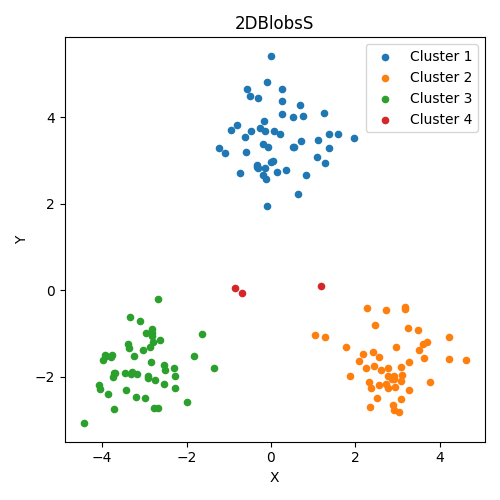
\includegraphics[width=\myimgwidth]{images/datasets/2DBlobsS.png}
    \caption{2DBlobsS.}
    \label{fig:2DBlobsS}
\end{wrapfigure}
The \textbf{2DBlobsS} dataset (Figure \ref{fig:2DBlobsS}) is a synthetic two-dimensional dataset consisting of three compact Gaussian clusters (blue, orange, and green) with no overlap. Each cluster contains densely concentrated points surrounding a central mean. Two additional points (red) are positioned between the clusters and are labeled as in-between instances (IBIs). These IBIs occupy intermediate positions in the feature space, capturing structural transitions between distinct clusters. The clear separation between clusters make this dataset a simple, low-complexity scenario for evaluating structure preservation in learned embeddings.
\newline

\begin{wrapfigure}{l}{\myimgwidth}
    \centering
    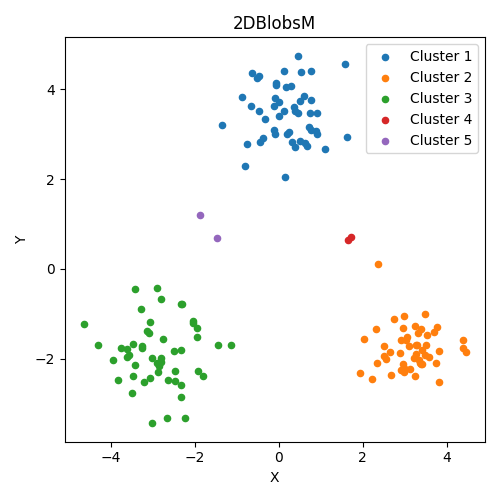
\includegraphics[width=\myimgwidth]{images/datasets/2DBlobsM.png}
    \caption{2DBlobsM.}
    \label{fig:2DBlobsM}
\end{wrapfigure}
The \textbf{2DBlobsM} dataset (Figure \ref{fig:2DBlobsM}) is a synthetic two-dimensional dataset composed of three primary Gaussian clusters, each depicted in a distinct color (blue, orange, and green). These clusters contain tightly grouped data points distributed around separate centroids. In addition to the main clusters, there are two pairs of points (red and purple) located between the clusters. These points are designated as in-between instances (IBIs), approximately equidistant from two clusters. This spatial configuration makes the dataset suitable for testing the ability to preserve both cluster integrity and multiple transitional relationships in the latent space.
\newline
\newpage

\begin{wrapfigure}{r}{\myimgwidth}
    \centering
    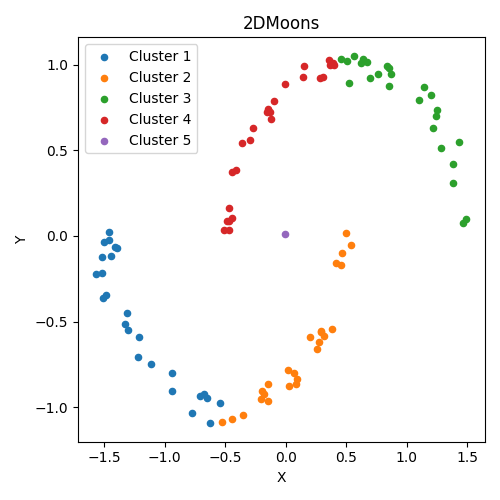
\includegraphics[width=\myimgwidth]{images/datasets/2DMoons.png}
    \caption{2DMoons.}
    \label{fig:2DMoons}
\end{wrapfigure}
The \textbf{2DMoons} dataset (Figure \ref{fig:2DMoons}) is a synthetic two-dimensional dataset composed of two interleaving half-moon–shaped clusters arranged in a nonlinear configuration. Each cluster is subdivided into two labeled segments (blue–orange and green–red) to facilitate analysis of local structure. A single point (purple) is located between the arcs and designated as an in-between instance (IBI), meaning it shares spatial proximity to both curved manifolds. The dataset’s non-linear topology and minimal number of IBIs make it a challenging case for dimensionality reduction methods that aim to preserve both manifold geometry and transitional points.
\newline

\begin{wrapfigure}{l}{\myimgwidth}
    \centering
    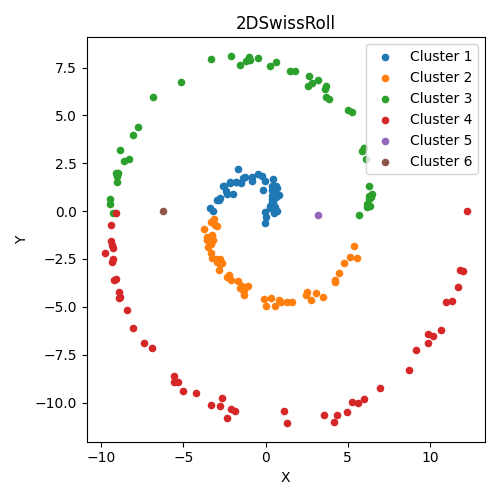
\includegraphics[width=\myimgwidth]{images/datasets/2DSwissRoll.png}
    \caption{2DSwissRoll.}
    \label{fig:2DSwissRoll}
\end{wrapfigure}
The \textbf{2DSwissRoll} dataset (Figure \ref{fig:2DSwissRoll}) is a synthetic two-dimensional dataset representing an rolled spiral manifold. The continuous spiral is segmented into contiguous curved sections (blue, orange, green, and red). Additional points (purple and brown) are placed between the main clusters and are labeled as in-between instances (IBIs). These IBIs lie along the spiral arms where neighboring sections meet, capturing transitional regions in the manifold’s geometry. The dataset’s continuous but highly non-linear structure makes it a strong benchmark for evaluating the ability to maintain neighborhood relationships and inter-cluster continuity.
\newline

\begin{wrapfigure}{r}{\myimgwidth}
    \centering
    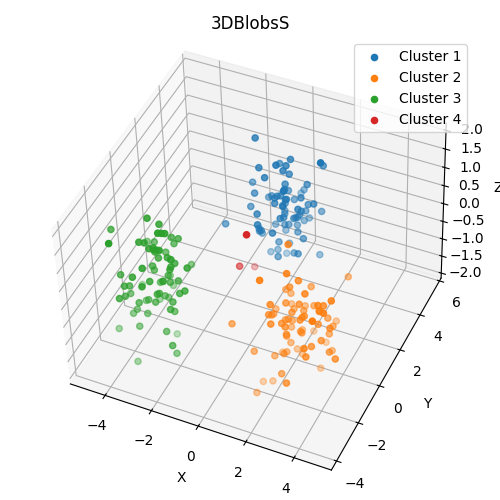
\includegraphics[width=\myimgwidth]{images/datasets/3DBlobsS.png}
    \caption{3DBlobsS.}
    \label{fig:3DBlobsS}
\end{wrapfigure}
The \textbf{3DBlobsS} dataset (Figure \ref{fig:3DBlobsS}) is a synthetic three-dimensional dataset composed of three compact Gaussian clusters (blue, orange, and green) arranged with no spatial overlap. Three additional points (red) are placed between the primary clusters and are labeled as in-between instances (IBIs). These IBIs represent transitional samples that capture mixed characteristics from all clusters. The dataset’s relatively simple structure, low number of IBIs, and well-separated clusters provide a controlled environment for testing structure preservation and neighborhood fidelity.
\newline

\begin{wrapfigure}{l}{\myimgwidth}
    \centering
    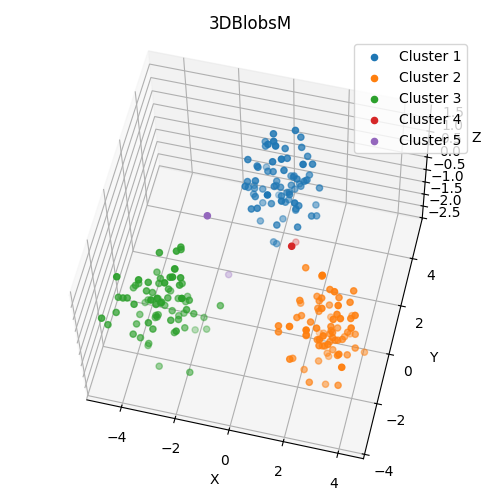
\includegraphics[width=\myimgwidth]{images/datasets/3DBlobsM.png}
    \caption{3DBlobsM.}
    \label{fig:3DBlobsM}
\end{wrapfigure}
The \textbf{3DBlobsM} dataset (Figure \ref{fig:3DBlobsM}) is a synthetic three-dimensional dataset generated from Gaussian distributions. It contains three main clusters (blue, orange, and green), each centered at distinct locations in the feature space. Two additional pairs of points (red and purple) are positioned in regions between the clusters and are designated as in-between instances (IBIs). These IBIs are situated approximately equidistant from multiple cluster centroids, forming transitional data points that share attributes of more two clusters. The dataset’s moderate complexity makes it suitable for evaluating how well the models preserve both distinct cluster boundaries and transitional relationships in low-dimensional embeddings.
\newline

\begin{wrapfigure}{r}{\myimgwidth}
    \centering
    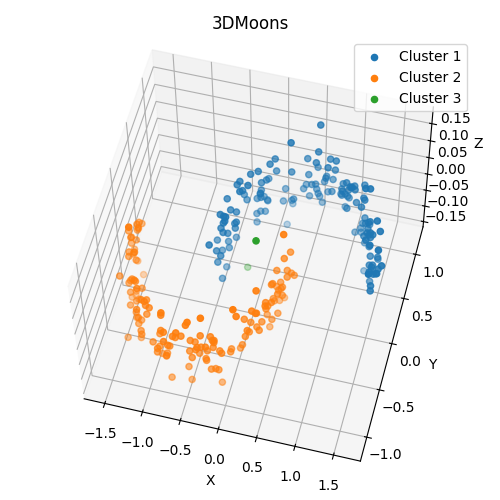
\includegraphics[width=\myimgwidth]{images/datasets/3DMoons.png}
    \caption{3DMoons.}
    \label{fig:3DMoons}
\end{wrapfigure}
The \textbf{3DMoons} dataset (Figure \ref{fig:3DMoons}) is a synthetic three-dimensional dataset characterized by two moon-shaped clusters (blue and orange). A single point (green) is placed between the two moons and labeled as an in-between instance (IBI). This IBI occupies a region of balanced proximity to both moons, representing a transitional point between distinct curved manifolds. The dataset’s non-linear geometry, combined with its minimal number of IBIs, makes it an effective benchmark for testing the ability to capture manifold structure and preserve transitional instances.
\newline

\begin{wrapfigure}{l}{\myimgwidth}
    \centering
    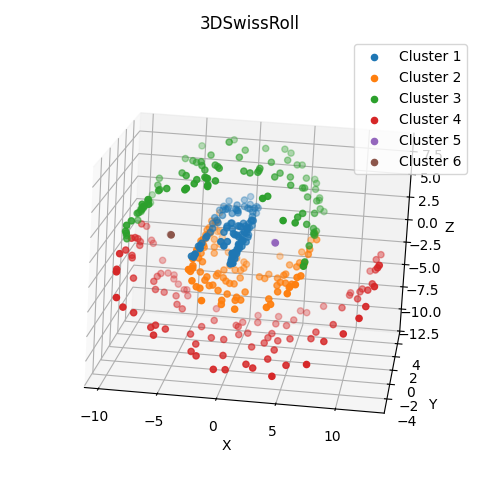
\includegraphics[width=\myimgwidth]{images/datasets/3DSwissRoll.png}
    \caption{3DSwissRoll.}
    \label{fig:3DSwissRoll}
\end{wrapfigure}
The \textbf{3DSwissRoll} dataset (Figure \ref{fig:3DSwissRoll}) is a synthetic three-dimensional dataset shaped as a rolled spiral manifold embedded in 3D space. The spiral is segmented into contiguous curved sections (blue, orange, green, and red). Several points (purple and brown) are positioned at boundary regions between clusters and are labeled as in-between instances (IBIs). These IBIs lie in areas where the manifold’s continuity creates local proximity between points from different labeled sections. The dataset’s highly non-linear geometry and mixed local–global proximity relationships make it a challenging benchmark for assessing neighborhood preservation and inter-cluster continuity.
\newline

\begin{wrapfigure}{r}{\myimgwidth}
    \centering
    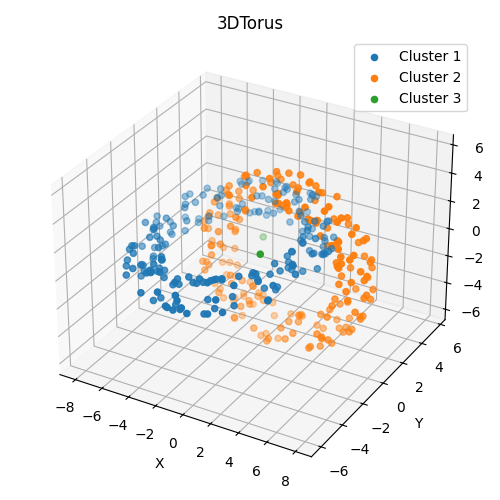
\includegraphics[width=\myimgwidth]{images/datasets/3DTorus.png}
    \caption{3DTorus.}
    \label{fig:3DTorus}
\end{wrapfigure}
The \textbf{3DTorus} dataset (Figure \ref{fig:3DTorus}) is a synthetic three-dimensional dataset featuring two ring-shaped clusters (blue and orange) arranged in a toroidal configuration. The rings are positioned in parallel, forming a closed-loop geometry. Two points (green) are placed between the two rings and designated as an in-between instance (IBI). This IBI represents a transitional sample that resides between distinct curved manifolds within the torus structure. The dataset’s global circular topology and localized inter-ring relationships make it suitable for testing the ability of embedding methods to preserve both geometric structure and transitional regions.
\newline

\begin{wrapfigure}{l}{\myimgwidth}
    \centering
    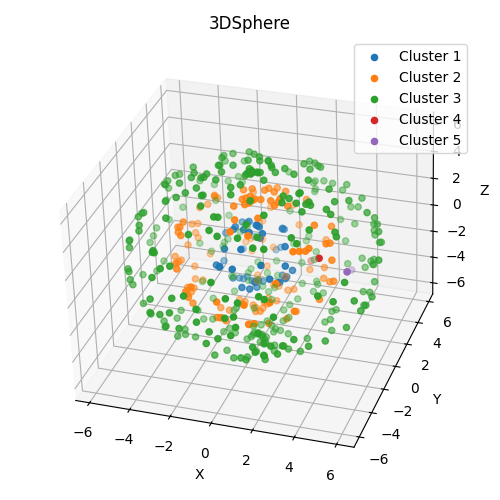
\includegraphics[width=\myimgwidth]{images/datasets/3DSphere.png}
    \caption{3DSphere.}
    \label{fig:3DSphere}
\end{wrapfigure}
The \textbf{3DSphere} dataset (Figure \ref{fig:3DSphere}) is a synthetic three-dimensional dataset consisting of three spherical clusters (blue, orange, and green) arranged as nested shells around a central origin. Points are uniformly distributed across each spherical surface. Additional points (red and purple) are positioned between these spherical shells and labeled as in-between instances (IBIs). These IBIs represent transitional samples located in intermediate radial zones, sharing spatial characteristics with multiple spherical layers. The dataset’s symmetric, non-linear geometry provides a robust test for evaluating global shape preservation and the accurate mapping of transitional points in reduced-dimensional representations.

\section{Autoencoder Framework} \label{sec:autoencoder_framework}

The framework of the autoencoders investigated in this thesis is structured around three central components, as outlined in Figure \ref{fig:roadmap}: architectural design, training stategy and loss configuration. These elements form the foundation for investigating how autoencoders can effectively capture in-between instances (IBIs) in high-dimensional data. While several hyperparameters are varied during experimentation, others are kept constant throughout. This setup provides a controlled yet flexible framework for assessing the impact of architectural and loss design choices. Each of these components is described in detail in the following sections.
\begin{figure}[ht]
    \centering
    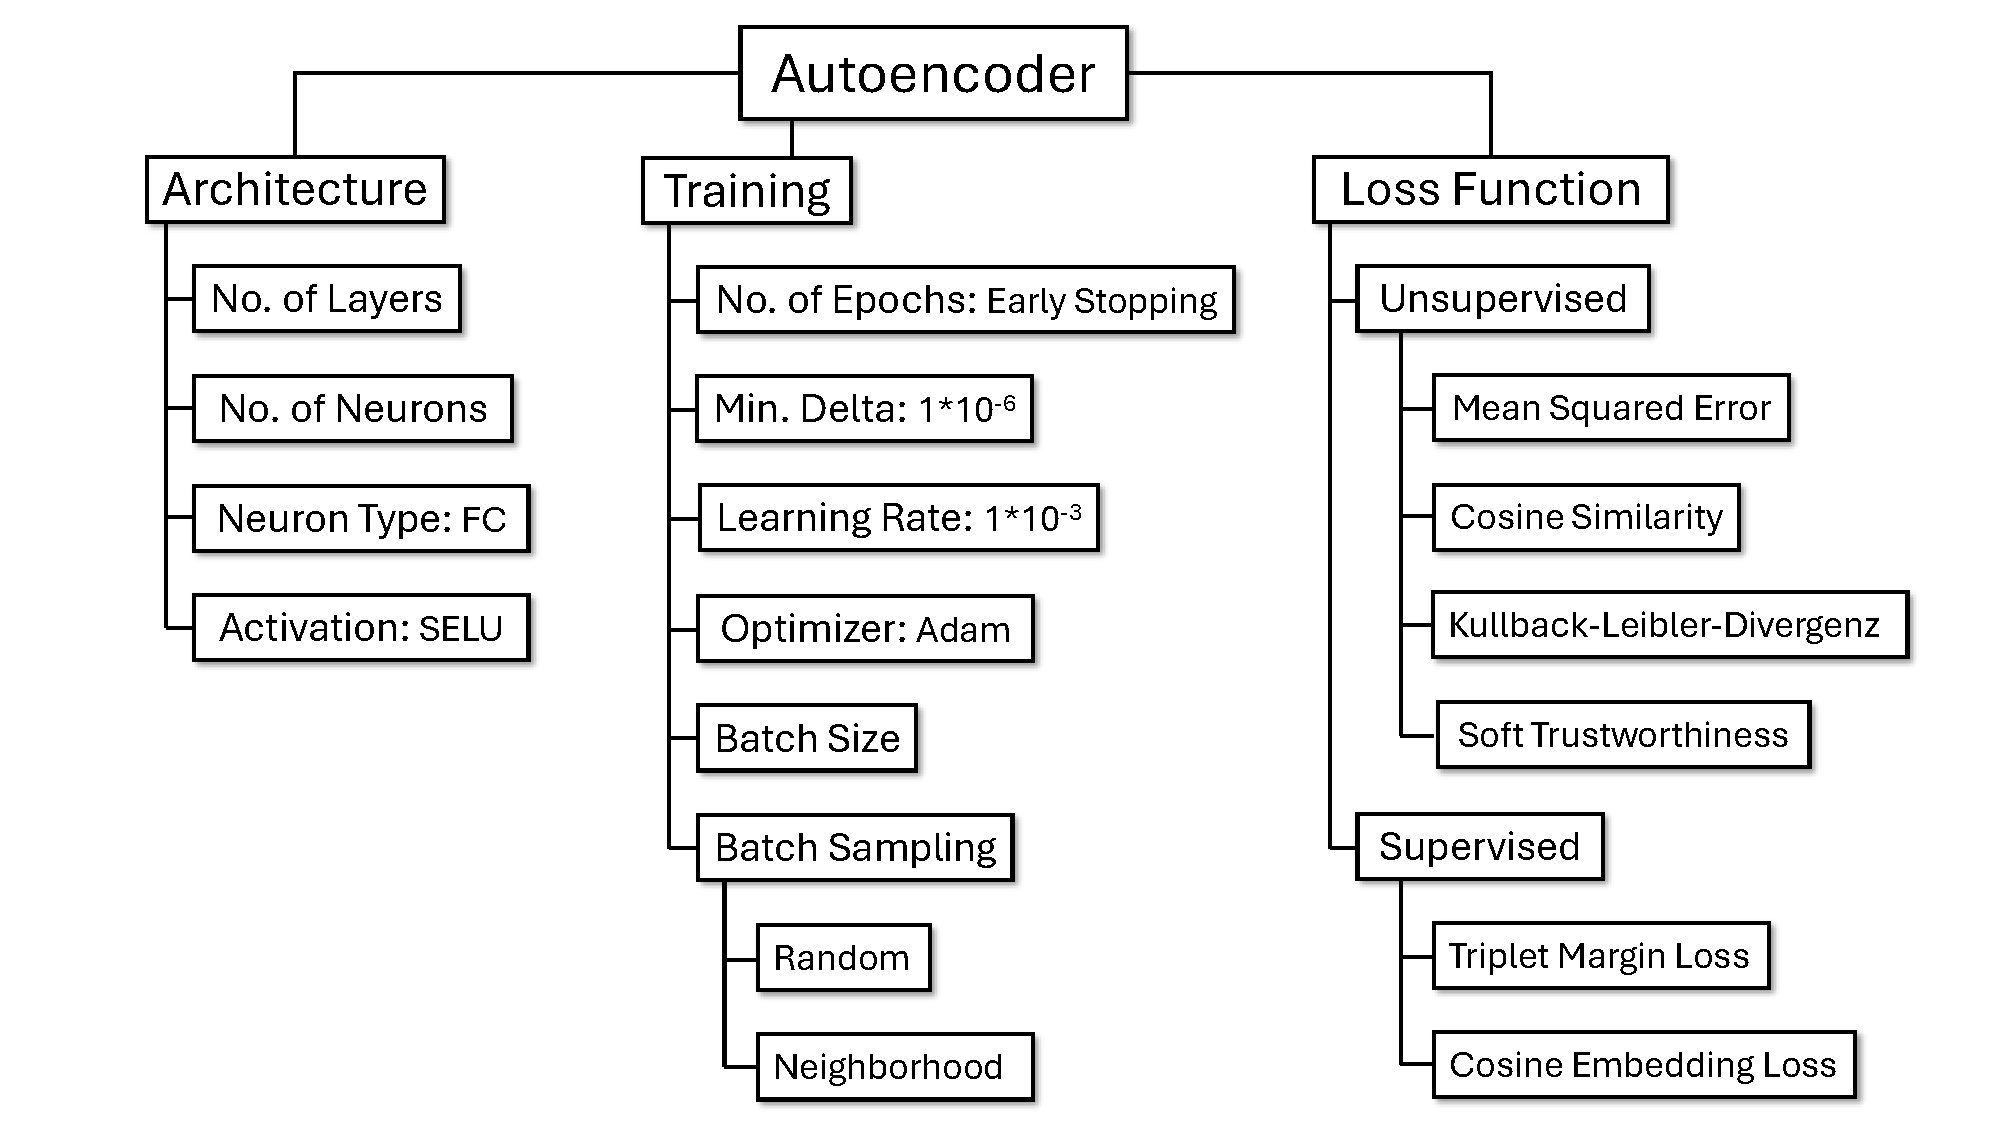
\includegraphics[width=\linewidth]{images/Roadmap.pdf}
    \caption{Overview of the framework, illustrating the three core components that guide the experimental design. Constant parameters are indicated accordingly. Inspired by \cite{Charte18}}
    \label{fig:roadmap}
\end{figure}

\subsection{Architecture and Training Strategy}

The performance and representational capacity of autoencoders are profoundly influenced by the architectural choices and training configurations employed during model development. This section outlines the specific design decisions made in constructing the autoencoder models used in this thesis. Additionally, it details key training parameters that directly impact the model’s convergence behavior and generalizability. Each choice is grounded in both theoretical considerations and empirical best practices, ensuring that the resulting autoencoder configurations are well-suited to capturing in-between instances (IBIs) while maintaining reconstruction fidelity and training stability.

\paragraph{Number of Epochs:} The number of epochs refers to the number of complete passes through the entire training dataset during the learning process. Selecting an appropriate number of epochs is critical, as it directly influences model performance and generalization. If the number of epochs is too low, the model may underfit, failing to capture meaningful patterns in the data. If too high, it risks overfitting, learning noise rather than underlying structure \cite{Berahmand24}. To mitigate this, all experiments will employ early stopping, a regularization technique that halts training when the validation performance ceases to improve beyond a defined threshold. Specifically, a minimum delta value of $1\cdot10^{-5}$ will be used to determine the smallest improvement in validation loss considered significant. If the improvement falls below this threshold for a set number of epochs, training is terminated early. This approach ensures a balanced training process, promoting both efficiency and generalizability across different configurations and datasets.

\paragraph{Neuron Type:} Neuron types vary based on the specific computational roles they fulfill. Fully connected neurons, fundamental to traditional multilayer perceptrons, are characterized by each neuron in one layer being connected to every neuron in the subsequent layer, allowing for rich, but often computationally intensive, interactions across the network. Convolutional neurons are structured to exploit spatial hierarchies by processing data through localized receptive fields using shared weights, making them particularly effective for image and pattern recognition tasks. Recurrent neurons introduce a temporal dimension by incorporating feedback loops that allow information to persist across time steps, enabling the modeling of sequential data such as language or time series [\cite{Berahmand24}, \cite{Charte18}]. However, for all experiments in this study, we exclusively employ fully connected neurons, as our data does not involve sequential or image-based features and thus does not require the specialized processing capabilities of convolutional or recurrent architectures.

\paragraph{Learning Rate:} The learning rate is a critical hyperparameter that governs the magnitude of weight updates during training, directly influencing the speed and stability of the optimization process. It determines how much the model's parameters are adjusted in response to the calculated error from each iteration of backpropagation. A learning rate that is too high can cause the model to overshoot minima in the loss landscape, potentially leading to divergence or oscillation rather than convergence. Conversely, a learning rate that is too low may result in excessively slow training and an increased risk of becoming trapped in local minima or saddle points. Adaptive optimization algorithms, dynamically adjust the rate during training to balance convergence speed with stability [\cite{Berahmand24}, \cite{Charte18}]. In our experiments the initial learning rate is set to $1\cdot10^{-3}$.

\paragraph{Optimization Algorithm:} Optimization algorithms are fundamental to training machine learning models, as they govern how model parameters are updated to minimize a loss function. Stochastic Gradient Descent (SGD) is one of the simplest and most widely used optimization methods. It updates parameters by computing the gradient of the loss with respect to the parameters using a randomly selected subset of data, introducing noise that can help escape local minima. However, SGD can be inefficient, especially in scenarios involving sparse data or ill-conditioned loss landscapes. To address such limitations, adaptive learning rate methods have been developed. AdaGrad \cite{Adagrad}, for instance, adapts the learning rate for each parameter individually by accumulating the square of past gradients, which improves performance on sparse data but can lead to overly small learning rates over time. RMSProp \cite{RMSProp} modifies AdaGrad by using an exponentially decaying average of squared gradients, preventing the learning rate from diminishing too quickly and thereby maintaining consistent progress. Building upon both RMSProp and momentum-based updates, Adam (Adaptive Moment Estimation) \cite{Adam} computes adaptive learning rates using estimates of the first and second moments of the gradients \cite{Berahmand24}. By combining the benefits of RMSProp and momentum, Adam tends to perform robustly across a wide range of deep learning tasks \cite{Charte18}. Due to its efficiency and strong empirical performance, we will employ the Adam optimizer in all our experiments.

\paragraph{Batch Size:} The batch size, the number of samples processed before updating model parameters, significantly influences both training efficiency and model performance. Smaller batch sizes result in more frequent updates, which can help the model escape local minima, potentially enhancing generalization. However, these frequent updates introduce greater noise into the gradient estimates, which may destabilize training and slow overall progress. In contrast, larger batch sizes yield more stable and accurate gradient estimates, enabling faster convergence, though they demand more memory. Selecting an optimal batch size is highly context-dependent, influenced by the model architecture, dataset characteristics, and hardware constraints \cite{Berahmand24}. Consequently, in this work, the batch size will be treated as a variable hyperparameter, systematically varied and tested across experiments to assess its impact on training dynamics and generalization performance.

\paragraph{Batch Sampling:} Batch sampling refers to the process of selecting subsets of data points from the full training dataset to compute gradients and update model parameters during training. Traditionally, batches are sampled randomly, ensuring that each mini-batch represents a diverse mix of the data distribution, which helps improve generalization \cite{LeCun12}. However, alternative strategies like neighborhood sampling have gained attention, particularly in domains such as graph neural networks \cite{Hamilton18}, where local context plays a significant role. Neighborhood sampling involves selecting data points that are close to each other in some feature space or topological structure, thereby preserving local correlations and potentially enhancing learning from structured or spatially coherent data. The choice between random and neighborhood sampling is not arbitrary and should be informed by the nature of the loss function used in the experiments. If the loss is global, aggregating information across the entire dataset, random sampling is generally more appropriate. In contrast, if the loss function emphasizes local patterns or relationships, neighborhood sampling can provide more relevant gradient updates. Thus, sampling strategy must be aligned with the scope of the loss function to optimize learning efficacy.

\paragraph{Activation Function:} Activation functions (Table \ref{tab:activations_functions}) are a critical component in artificial neural networks, including autoencoders, where they endow the model with the capacity to capture and learn complex, non-linear relationships in data. These functions operate by transforming the weighted sum of inputs into a node’s output, introducing non-linearity into the model’s computations. Without them, a network composed of only linear operations would be functionally equivalent to a linear model. Among the most commonly used activation functions in autoencoders are the sigmoid and hyperbolic tangent (tanh), both of which are bounded. The sigmoid maps input values to the range [0, 1], while tanh spans [-1, 1], often resulting in stronger gradients and better convergence \cite{Berahmand24}. Rectified Linear Units (ReLU) \cite{ReLU} are also widely used due to their simplicity, although their tendency to output zero for negative inputs can hinder the reconstruction performance in some autoencoder configurations \cite{Charte18}. To address this, more advanced variants like the Scaled Exponential Linear Unit (SELU) \cite{SELU} have been developed, which can maintain a healthy flow of gradients. Given SELU’s benefits, we will therefore be using it as the activation function in our experiments to enhance the reconstruction fidelity.

\begin{table}[ht]
\centering
\renewcommand{\arraystretch}{1.5} % More row height
\begin{tabular}{|
  >{\centering\arraybackslash}m{3cm} |
  >{\centering\arraybackslash}m{5cm} |
  >{\centering\arraybackslash}m{1.33cm} |
  >{\centering\arraybackslash}m{4cm} |}
\hline
\textbf{Name} & \textbf{Equation} & \textbf{Output} & \textbf{Curve}\\
\hline
\textbf{Sigmoid} & $f(x) = \frac{1}{1 + e^{-x}}$ & $[0, 1]$ & 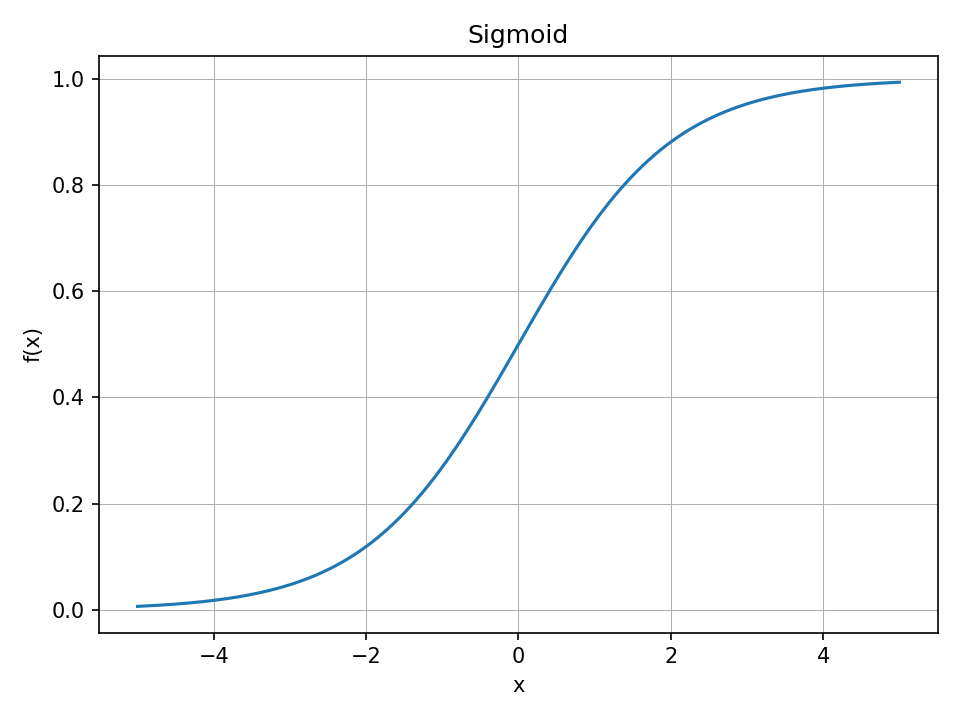
\includegraphics[width=4cm]{images/sigmoid.png}\\
\hline
\textbf{Tanh} (Tangens hyperbolicus) & $f(x) = \frac{e^x - e^{-x}}{e^x + e^{-x}}$ & $[-1, 1]$ & 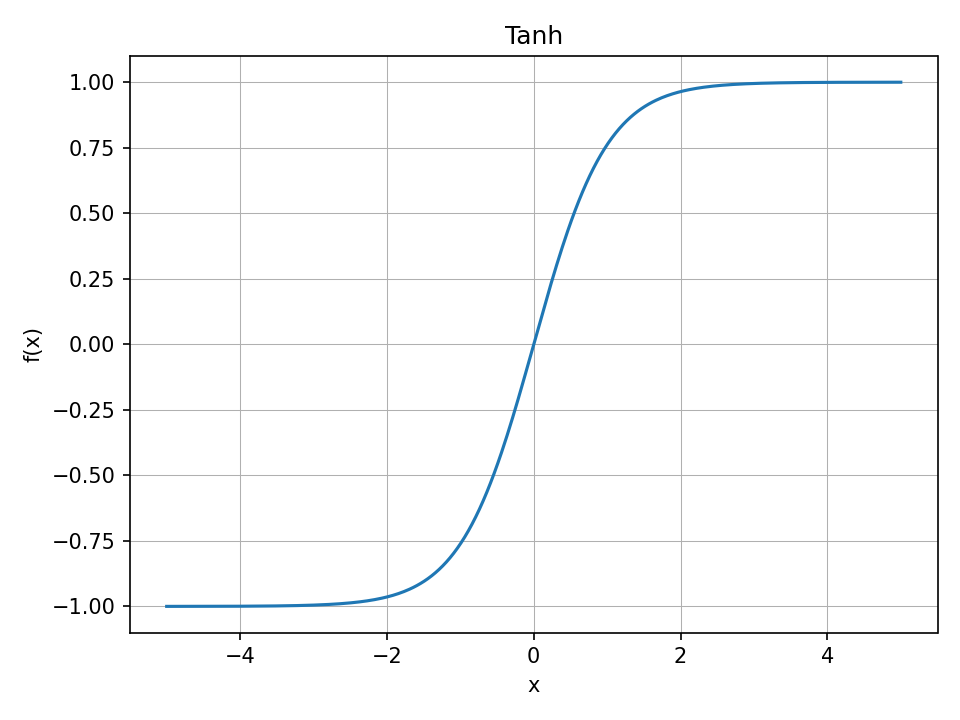
\includegraphics[width=4cm]{images/tanh.png}\\
\hline
\textbf{ReLU} (Rectified Linear Unit) & $f(x) = \max(0, x)$ & $[0, \infty]$ & 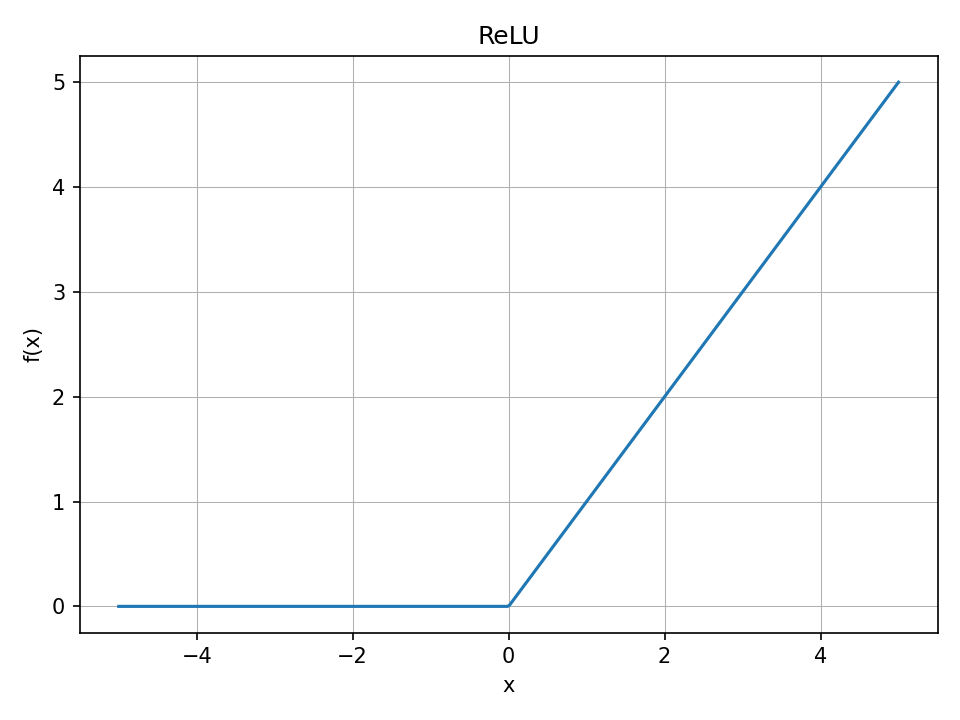
\includegraphics[width=4cm]{images/relu.png}\\
\hline
\textbf{SELU} (Scaled Exponential Linear Unit) & 
$f(x) = \lambda\begin{cases} 
x & \text{if } x > 0 \\
\alpha e^x - \alpha & \text{if } x \leq 0 
\end{cases}$ & $[-2, \infty]$ & 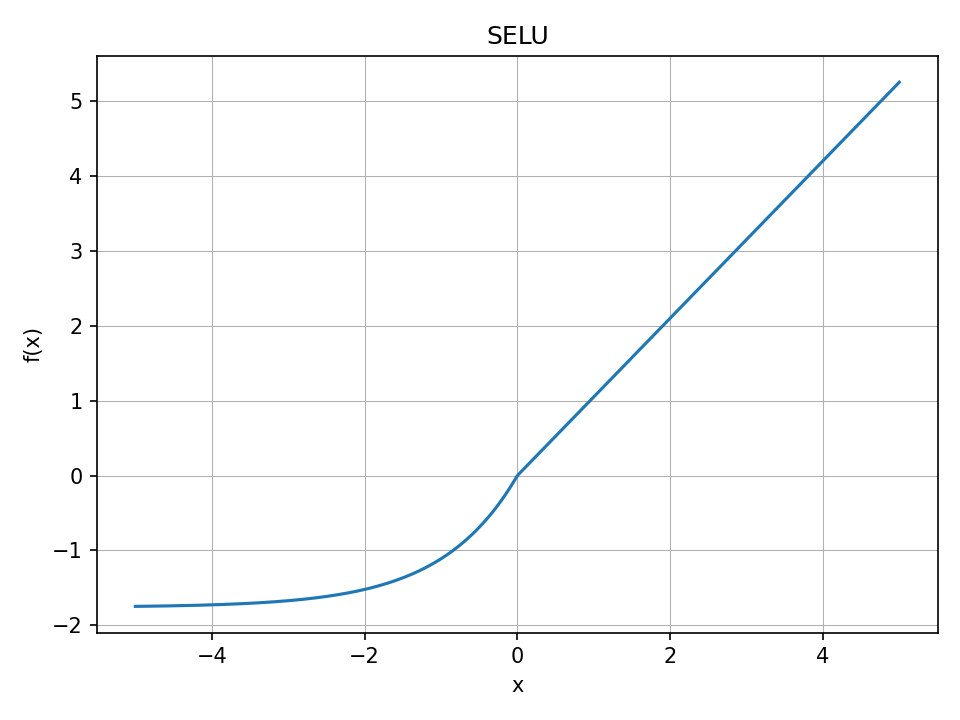
\includegraphics[width=4cm]{images/selu.png}\\
\hline
\end{tabular}
\caption{Activation Functions. Adapted from \cite{Berahmand24}}
\label{tab:activations_functions}
\end{table}

\paragraph{Number of Layers:} The number of layers in an autoencoder plays a critical role in determining its capacity to learn meaningful representations of input data. The depth of the network, defined by the number of layers, affects both the expressiveness and the generalization ability of the model. Shallow autoencoders, with only one or two hidden layers, may suffice for simple or low-dimensional data, offering computational efficiency and reduced risk of overfitting \cite{Berahmand24}. In contrast, deep autoencoders, which comprise multiple hidden layers in both the encoder and decoder, are better suited for capturing complex, hierarchical features, especially in high-dimensional datasets. However, increasing the number of layers also introduces challenges, including vanishing gradients, longer training times, and a higher demand for regularization techniques \cite{Charte18}. Because the optimal number of layers depends on the data characteristics and task complexity, we will first identify a suitable network depth through preliminary experiments before proceeding with further evaluations \cite{Goodfellow16}.

\paragraph{Number of Neurons per Layer:} The number of neurons in each layer is typically dictated by the dimensionality of the data. The input layer contains a number of neurons equal to the number of features in the input data, ensuring that each input dimension is represented. The output layer mirrors the input layer in size, especially in basic autoencoders, since the goal is to reconstruct the input from a compressed representation. Hidden layers, particularly the bottleneck or latent space layer, contain fewer neurons than the input or output layers to enforce dimensionality reduction. Additional hidden layers may exist in deeper autoencoders, often arranged symmetrically around the bottleneck to form the encoder and decoder components. The specific number of neurons in these hidden layers typically decreases toward the bottleneck and then increases symmetrically in the decoder \cite{Charte18}.

\paragraph{Size of Latent Space:} The size of the latent space in autoencoders plays a critical role in determining the model’s capacity to compress and reconstruct data effectively. A smaller latent space forces the model to learn more compact and informative representations by distilling the most salient features of the input data, which can enhance generalization and denoising performance but may also lead to underfitting if important information is lost. Conversely, a larger latent space allows for more detailed encoding of the input, potentially improving reconstruction fidelity but increasing the risk of overfitting, where the model memorizes rather than generalizes. The optimal size of the latent space is highly dependent on the complexity and intrinsic dimensionality of the data \cite{Berahmand24}. For the purposes of our experiments, we will use latent space sizes of 2 and 3, which, while relatively small, are particularly advantageous for visualization, allowing the encoded representations to be easily interpreted and plotted in two- or three-dimensional space.

\subsection{Loss Configurations}

Loss functions form the mathematical foundation for training neural networks by providing a quantitative measure of the model’s performance on a given task. In the context of autoencoders loss functions guide the optimization of two key components: the encoder and the decoder. The \emph{encoder}, denoted by a parametric function \( f_\theta: \mathbb{R}^n \rightarrow \mathbb{R}^m \), maps an input \( x \in \mathbb{R}^n \) to a lower-dimensional latent representation \( h = f_\theta(x) \). The \emph{decoder}, represented by \( g_\phi: \mathbb{R}^m \rightarrow \mathbb{R}^n \), attempts to reconstruct the original input from the latent code, yielding a reconstruction \( \hat{x} = g_\phi(h) = g_\phi(f_\theta(x)) \). The loss function \( \mathcal{L}: \mathbb{R}^n \times \mathbb{R}^n \rightarrow \mathbb{R}_{\geq 0} \) measures the discrepancy between the original input \( x \) and its reconstruction \( \hat{x} \), with the objective of minimizing this difference across the dataset. Formally, the training process seeks the parameters \( \theta \) and \( \phi \) that minimizes the loss. Different loss functions impose different assumptions on the data distribution and can be chosen to emphasize specific characteristics of the reconstruction. In the sections that follow, various loss functions will be introduced in terms of their mathematical formulation and practical relevance to training effective autoencoder models.

\paragraph{Mean Squared Error:} The Mean Squared Error (MSE) is a widely used loss function in autoencoders [\cite{Berahmand24}, \cite{Charte18}]. It evaluates the average of the squared differences between each input feature and its corresponding reconstruction. This squared formulation ensures that larger errors are penalized more heavily than smaller ones, encouraging the model to prioritize accurate reconstructions across all dimensions. Mathematically the MSE is defined as
\[
\mathcal{L}_{MSE}(x, \hat{x}) = \|x - \hat{x}\|^2_2 = \frac{1}{n}\sum_{i=1}^{n} (x_i - \hat{x}_i)^2 \ \cite{torch.nn}.
\]

\paragraph{Cosine Similarity:} Cosine similarity is a metric not frequently employed in the context of autoencoders. It measures the angular distance between two vectors in a high-dimensional space, offering a geometry-based assessment of similarity that is invariant to vector magnitude. In applications involving information retrieval tasks, cosine similarity serves as a valuable tool for comparing embeddings \cite{Xia15}. By focusing on the orientation rather than the length of the vectors, it effectively captures semantic closeness, which is especially useful when dealing with normalized feature representations. This becomes crucial in scenarios where the magnitude of embeddings may vary due to the nature of the data, but the directional alignment is preserved. Consequently, using cosine similarity in these scenarios allows autoencoders to be more robust in identifying relationships between inputs, enhancing the performance of tasks where understanding the relative positioning of data in feature space is more informative than absolute distances \cite{Zhang23}. Mathematically the cosine similarity is defined as
\[
\mathcal{L}_{CosSim}(x, \hat{x}) = \frac{x \cdot \hat{x}}{\|x\| \, \|\hat{x}\|} = \frac{\sum_{i=1}^{n} x_i \hat{x}_i}{\sqrt{\sum_{i=1}^{n} x_i^2} \cdot \sqrt{\sum_{i=1}^{n} \hat{x}_i^2}} \ \cite{torch.nn}.
\]

\paragraph{Kullback-Leibler Divergence:} The Kullback-Leibler Divergence (KL divergence) is a fundamental concept in information theory and plays a crucial role in neural networks, particularly in probabilistic models. It quantifies the discrepancy between two probability distributions and is often interpreted as the amount of information lost when an approximate distribution is used to represent a true distribution \cite{Kingma19}. In neural networks, KL divergence commonly appears in training objectives such as those for Variational Autoencoders (VAEs), where it acts as a regularization term that encourages the learned posterior to remain close to a prior distribution. In our case, however, we do not use the latent distributions of the KL divergence (as is standard in VAEs), but instead rely directly on the known probability densities of the samples. The form of the KL divergence, expressed as a loss function between the true distribution $p(x)$ and an approximate distribution $q(\hat{x})$, is given by:
\[
\mathcal{L}_{\text{KLD}}(x, \hat{x}) = p(x) \log \left( \frac{p(x)}{q(\hat{x})} \right) \ \cite{torch.nn}.
\]

\paragraph{Soft Trustworthiness:} The trustworthiness measure evaluates how accurately neighborhood relationships in a low-dimensional projection reflect the true proximities in the original high-dimensional data space. Specifically, it quantifies the degree to which the embedding introduces misleading neighbor relationships by including points that appear close in the projection but are actually distant in the original space. The trustworthiness score is calculated by identifying, for each data point, the projected neighbors that are not among its true nearest neighbors, and then summing the rank distances of these intruding points in the original space \cite{Venna01}. A lower cumulative error indicates a more trustworthy projection. This measure is scaled to fall between 0 and 1, where values closer to 1 signify higher trustworthiness. However, the original formulation of trustworthiness relies on discrete rank comparisons and set comparisons, which makes it non-differentiable and therefore unsuitable as a loss function in gradient-based optimization frameworks. To address this limitation, we developed a differentiable variant of the trustworthiness measure, enabling its integration into learning algorithms that optimize projection quality through gradient descent. Formally, for a neighborhood size $k$, the trustworthiness score is:
$$
T(k) \;=\; 1 \;-\;
\frac{2}{n\,k\,(2n-3k-1)}
\;\sum_{i=1}^{n}
\;\sum_{j \,\in\,N_i^k}
\bigl(r_X(i,j)\;-\;k\bigr) \ \cite{Venna01},
$$
where $N_i^k$ contains the "intrusions": points that appear among the $k$ nearest neighbors of sample $i$ in the embedding space $Z$ but not in the original space $X$, and $r_X(i,j)$ is the rank of point $j$ with respect to $i$ in the original space. This formulation ensures that $0 \le T(k) \le 1$, with higher values indicating greater fidelity of neighborhood preservation. 

To enable optimization via backpropagation, we present a novel, differentiable variant called the \textbf{Soft Trustworthiness}. In this formulation, discrete operations such as hard ranking and set membership are replaced by continuous approximations. The hard rank $r_X(i,j)$ is substituted with a \textbf{soft rank} $\widetilde r_X(i,j)$ computed via sigmoids:
$$
\widetilde r_X(i,j)
= 1 \;+\!
\sum_{\ell=1}^{n}
\sigma\!\left(\frac{D_X(i,j)\;-\;D_X(i,\ell)}{\tau_r}\right),
$$
$$
\text{where}
\quad
\sigma(x)=\frac{1}{1+e^{-x}}
,
\quad
D_X(i,j) = \|x_i - x_j\|_2
.
$$
A \textbf{soft top-$k$} membership weight $W_Z(i,j)$ is then defined using the same mechanism in the embedding space:
$$
W_Z(i,j) = \text{clamp}\left(\frac{k+1 - \widetilde r_Z(i,j)}{k},\, 0,\, 1\right)
$$
which smoothly approximates whether point $j$ belongs to the top-$k$ neighbors of $i$ in the embedding.
The final trustworthiness loss penalizes soft intrusions using a ReLU thresholded rank error:
$$
S_{i,j} \;=\;\bigl[k-\widetilde r_Y(i,j)\bigr]_{+},
\quad
[x]_{+}=\max(x,0),
$$
and aggregates the penalties across the batch:
$$
\mathcal L_{\rm softTW}(x, \hat{x})_k
= \frac{2}{n\,k\,(2n-3k-1)}\,
\sum_{i=1}^{n}\;\sum_{j=1}^{n}
\;S_{i,j}\;\bigl(1 - W_Z(i,j)\bigr).
$$
This differentiable formulation retains the conceptual structure of the original trustworthiness score but enables its use in learning objectives. As the temperature parameters $\tau_r$ and $\tau_s$ approach zero, the soft approximation converges to the original discrete version. With this contribution, we not only formalize a previously unpublished extension of the classic trustworthiness metric but also make it accessible for modern, gradient-based optimization techniques in representation learning.

\subsection{Supervised Extentions}

Supervised extensions enhance autoencoders by incorporating label information into training, guiding the model to learn embeddings that are both reconstructive and semantically meaningful. This is especially important for detecting in-between instances (IBIs), which exist between distinct clusters and are often overlooked by unsupervised methods. By introducing loss functions like triplet margin loss and cosine embedding loss, the model is encouraged to bring similar instances closer together and push dissimilar ones apart in the latent space. These supervised objectives promote better class separation and alignment, making the embeddings more suitable for tasks requiring fine-grained discrimination, such as IBI detection.

\paragraph{Triplet Margin Loss:} Triplet margin loss is a foundational component in deep metric learning, aiming to structure the embedding space such that samples from the same class are drawn closer together while those from different classes are pushed apart by at least a fixed margin \cite{Yang19}. For a given triplet consisting of an anchor $h_a$, a positive example $h_p$ from the same class, and a negative example $h_n$ from a different class, the loss function encourages the squared distance between the anchor and the positive to be smaller than the squared distance between the anchor and the negative by a margin $m > 0$. This is mathematically formulated as
$$
\mathcal{L}_{\text{TriMarg}}(h) = \max\{0, \, \|h_a - h_p\|_2 - \|h_a - h_n\|_2 + m \} \ \cite{torch.nn}.
$$
The incorporation of this loss steers the embedding space toward enhanced intra-class compactness and inter-class separability, which is particularly beneficial for distinguishing in-between instances.

\paragraph{Cosine Embedding Loss:} Cosine embedding loss is a metric learning objective commonly employed in tasks where understanding the similarity or dissimilarity between paired data points is crucial \cite{Singh18}. It evaluates how closely the angular relationship between two feature representations aligns with a target label. Given two vectors $h_i$ and $h_j$, and a label $y \in \{1, -1\}$ indicating whether the pair is similar or dissimilar, the cosine embedding loss is expressed as
$$
\mathcal{L}_{\text{CosEmb}}(h) = 
\begin{cases}
1 - \cos(h_i, h_j), & \text{if } y = 1 \\
\max\{0, \cos(h_i, h_j) - m\}, & \text{if } y = -1
\end{cases}
\ \cite{torch.nn},
$$
where $\cos(h_i, h_j) = \dfrac{h_i \cdot h_j}{\|h_i\| \|h_j\|}$ denotes the cosine similarity between the two vectors, and $m \in [0,1]$ is a margin that defines the maximum allowable similarity for dissimilar pairs. This loss encourages the model to generate embeddings that are directionally aligned when the inputs are semantically similar and angularly separated beyond the margin when they are not. Unlike the triplet margin loss, which requires triplet sampling, the cosine embedding loss functions on pairs, simplifying the sampling strategy while still enforcing semantic alignment.

\section{Evaluation Protocol}

The evaluation strategy adopted in this thesis relies on two principal methods: the quantitative analysis of loss values and the qualitative visual examination of the latent space. While both approaches contribute to understanding the performance of the autoencoder models, the visual analysis is considered the more informative and decisive component, particularly in the context of in-between instance (IBI) preservation.

Quantitative evaluation is carried out by monitoring loss values during training, using the specific objective functions associated with each experiment. While these metrics quantify the reconstruction fidelity or embedding structure in a mathematically rigorous way, their absolute values are not directly comparable across different loss functions due to differing scales and underlying assumptions. Moreover, a lower loss value does not necessarily imply improved IBI preservation, as the objectives may prioritize reconstruction accuracy or local neighborhood preservation without explicitly considering inter-cluster instances.

Given these limitations, greater emphasis is placed on visual examination of the latent representations produced by the autoencoders. Since all experiments constrain the latent space to two or three dimensions, the resulting embeddings can be plotted directly and interpreted visually. These visualizations provide critical insight into the geometric structure of the encoded data, such as the separation of clusters, the continuity of transitions between them, and the presence of points situated between distinct groupings. Patterns that are difficult to capture through scalar loss values, such as overlapping cluster boundaries or emerging bridges between classes, are often readily apparent through visual inspection.

Therefore, while loss values serve as a basic sanity check for training convergence and model stability, it is the qualitative structure of the latent space, revealed through visual analysis, that ultimately guides the interpretation of IBI preservation and model effectiveness in this study.

\section{Tools and System Specifications}

The computational experiments conducted in this thesis were performed on a high-performance desktop system running Windows 11 Pro 64-bit. The system was equipped with an AMD Ryzen 7 3700X processor, featuring eight cores operating at a base clock speed of 3.6 GHz. This multi-core architecture provided the parallel processing capabilities necessary to efficiently handle the training of deep neural networks, especially in the context of the iterative optimization routines required for autoencoder models. The system was also outfitted with 32 GB of DDR4 RAM clocked at 3.2 GHz, which ensured that the datasets and neural network parameters could be stored in memory without incurring performance bottlenecks. Although the machine included an NVIDIA GeForce GTX 1660 SUPER graphics card, no GPU acceleration was utilized during the training or evaluation of the models.

The entire software environment was implemented using Python 3.12.9 \cite{Python}, a language widely adopted in scientific computing and machine learning for its robust ecosystem and extensive library support. Core computational and visualization tasks were facilitated by several key libraries. NumPy 2.1.3 \cite{NumPy} was employed for numerical operations, particularly for managing multi-dimensional arrays and performing vectorized computations central to data preprocessing and loss function calculations. Matplotlib 3.10.0 \cite{Matplotlib} served as the primary tool for plotting, enabling visual inspection of reconstruction fidelity and latent space structures. Most crucially, PyTorch 2.5.1 \cite{PyTorch} was used as the deep learning framework for building, training, and evaluating the autoencoder architectures. PyTorch offers seamless integration with NumPy, making it particularly suitable for research scenarios that require experimentation with novel loss functions.